\documentclass[11pt,a4paper]{article}
\usepackage[utf8]{inputenc}
\usepackage{amsmath}
\usepackage{amsfonts}
\usepackage{amssymb}
\usepackage{graphicx}
\usepackage{hyperref}
\usepackage{verbatim}
\usepackage[margin=.75in]{geometry}
\usepackage{listings} % for formatting code
\lstset
{
    language=Python,
    basicstyle=\footnotesize\ttfamily,
    numbers=left,
    stepnumber=1,
    showstringspaces=false,
    tabsize=4,
    breaklines=true,
    breakatwhitespace=false,
}

\setlength\parindent{0pt} % Removes all indentation from paragraphs

\author{Nikola Janju\v{s}evi\'{c}}
\title{ECE471, Selected Topics in Machine Learning \\ Midterm}

\begin{document}
\begin{large}
ECE471, Selected Topics in Machine Learning -- Midterm \\
\end{large}
Learning to See in the Dark \\
Nikola Janju\v{s}evi\'{c} \\
\today

\section*{Goal}
This assignment was an attempt to replicate the results of the paper: Learning to See in the Dark [1], in which the group trains a fully convolutional neural network to infer a properly exposed RGB image from an input, severely underexposed, RAW image. The Seeing in the Dark (SID) group's code can be seen at \url{https://github.com/cchen156/Learning-to-See-in-the-Dark}

\section*{Remarks}
RAW files are {\Large large}. I decided to decimate my input RAW files and ground truth PNGs by a factor of 16 so that all the training images could be easily loaded into memory. It is possible that this decimation ruins the set up that makes the SID group's results possible, namely, the spatial context from the original RAW file may be lost.

\section*{Sad (approaching not sad) Results}
After 100+ epochs, my network stagnated, producing only brown squares. I then changed some hyper parameters around, including input patch-size, activation function, kernel initialization, and annealed learning rates. I was then able to train to a much lower average cost, but the model still stagnates at a relatively high value. Further investigation is needed to train further. My next step, if time was permitting, would be to apply further data-augmentation (as performed in the paper). \textbf{Note}: input images are not shown as they are essentially black to the human eye. \\
\begin{figure}[h]
	\centering
	
\includegraphics[width=.25\textwidth]{../logs/0090_RELU6.jpg}
	\caption{20 epochs, activation fcn: relu6, patch-size: 32}
\end{figure}
\begin{figure}[h]
	\centering
	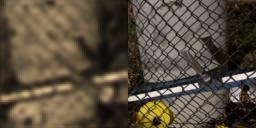
\includegraphics[width=.25\textwidth]{../logs/0040_RELUX.jpg}
	\caption{40 epochs, activation fcn: relu, xavier init, patch-size: 64}
\end{figure}
\begin{figure}[h]
	\centering
	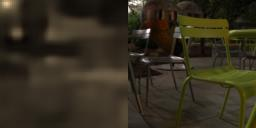
\includegraphics[width=.25\textwidth]{../logs/0100_CHAIR.jpg}
	\caption{100 epochs, activation fcn: relu, xavier init, patch-size: 64}
\end{figure}

\section*{References}
[1] Chen Chen, Qifeng Chen, Jia Xu, and Vladlen Koltun, "Learning to See in the Dark", in CVPR, 2018. \url{https://arxiv.org/pdf/1805.01934.pdf}

\pagebreak
\section*{Program: \texttt{sid2.py}}

\lstinputlisting[language=Python]{../sid2.py}

\pagebreak

\end{document}